\documentclass[11pt]{article}
\usepackage{preamble}
\usepackage{gset}
\def\week{5}
\def\theproblem{К\week.\arabic{problem}}
\begin{document}


\setcounter{problem}{0}
\def\theproblem{Д\week.\arabic{problem}}
{\textbf{\large Дискретная математика}\hfill \textbf{(Основной поток)}

\medskip %

\textbf{Домашнее задание \week}}

\medskip

\textbf{Дайте обоснованные ответы на следующие вопросы.}


\vspace{5mm}

\p Имеется множество $U$, состоящее из $n$ элементов. Сколькими способами можно выбрать в $U$ два подмножества $A$ и $B$ так, чтобы
\sp множества $A$ и $B$ не пересекались;
\sp множество $A$ содержалось бы в множестве $B$?
\sspace
а) Каждый элемент может быть в одном из 3 состояний:\sspace
1) Не входит в А, не входит в В\\
2) Входит в А, не входит в В\\
3) Входит в В, не входит в А \sspace

Элемент не может входить как в А, так и в В, потому что тогда пересечение этих множеств не будет пустым. Итого получаем по 3 независимых комбинации для каждого элемента, поэтому количество всех способов $3^{|U|}$
\sspace
\answer{$3^{|U|}$}
\sspace

\p Найдите количество таких путей из $(0,0)$ в $(n,n)$, что каждый шаг  либо $(1,0)$, либо $(0,1)$,  и в любой точке $(x,y)$ пути выполняется неравенство $|x-y|\leq1$.
\sspace
Для большей наглядности я привел изображение. 

\[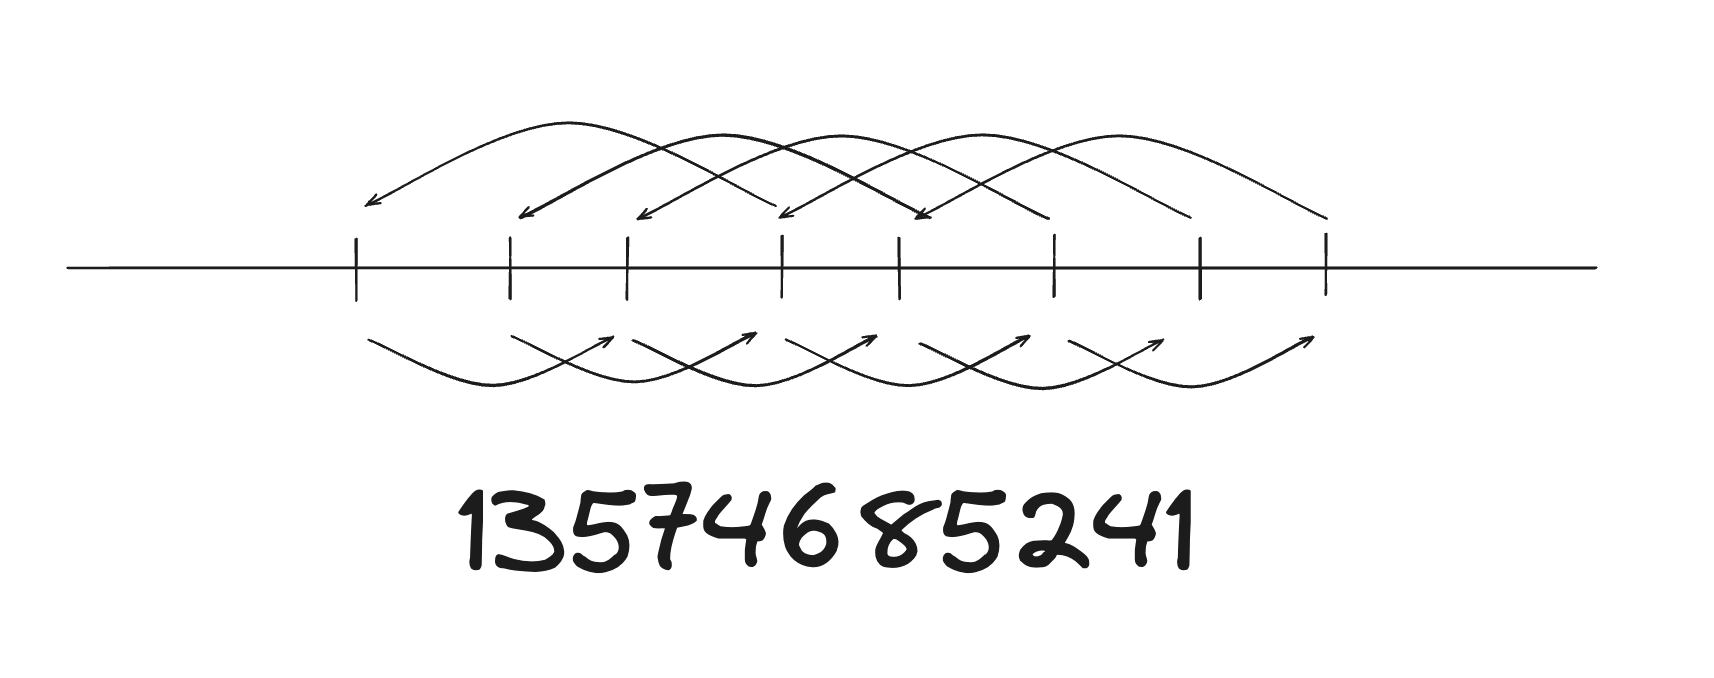
\includegraphics[width=125mm]{img}\]

Заметим, что из выполнения неравенства $|x-y|\leq1$ следует, что находясь в точке с координатами $(i, i)$ нельзя ходить 2 раза в одном направлении, потому что тогда модуль разницы координат будет равен 2. Это оначает, что находясь в точке $(i, i)$ через 2 хода можно оказаться только в точке $(i + 1, i + 1)$. Значит остается только посчитать количество возможных путей из $(i, i)$ в $(i + 1, i + 1)$. Их 2: либо сначала движение по горизонтали, затем по вертикали, либо сначала по вертикали, потом по горизонтали. Значит всего путей $2^n$, потому что есть 2 варианта на каждой клетке с координатами $(i,i), 0 \leq i < n$.
\sspace
\answer{$2^n$}
\sspace

\p Обозначим $Z_n$ количество двоичных слов длины $n$, в которых нет двух нулей подряд. Докажите, что $Z_n = F_{n+1}$ для всех $n\geq1$. \sspace

\[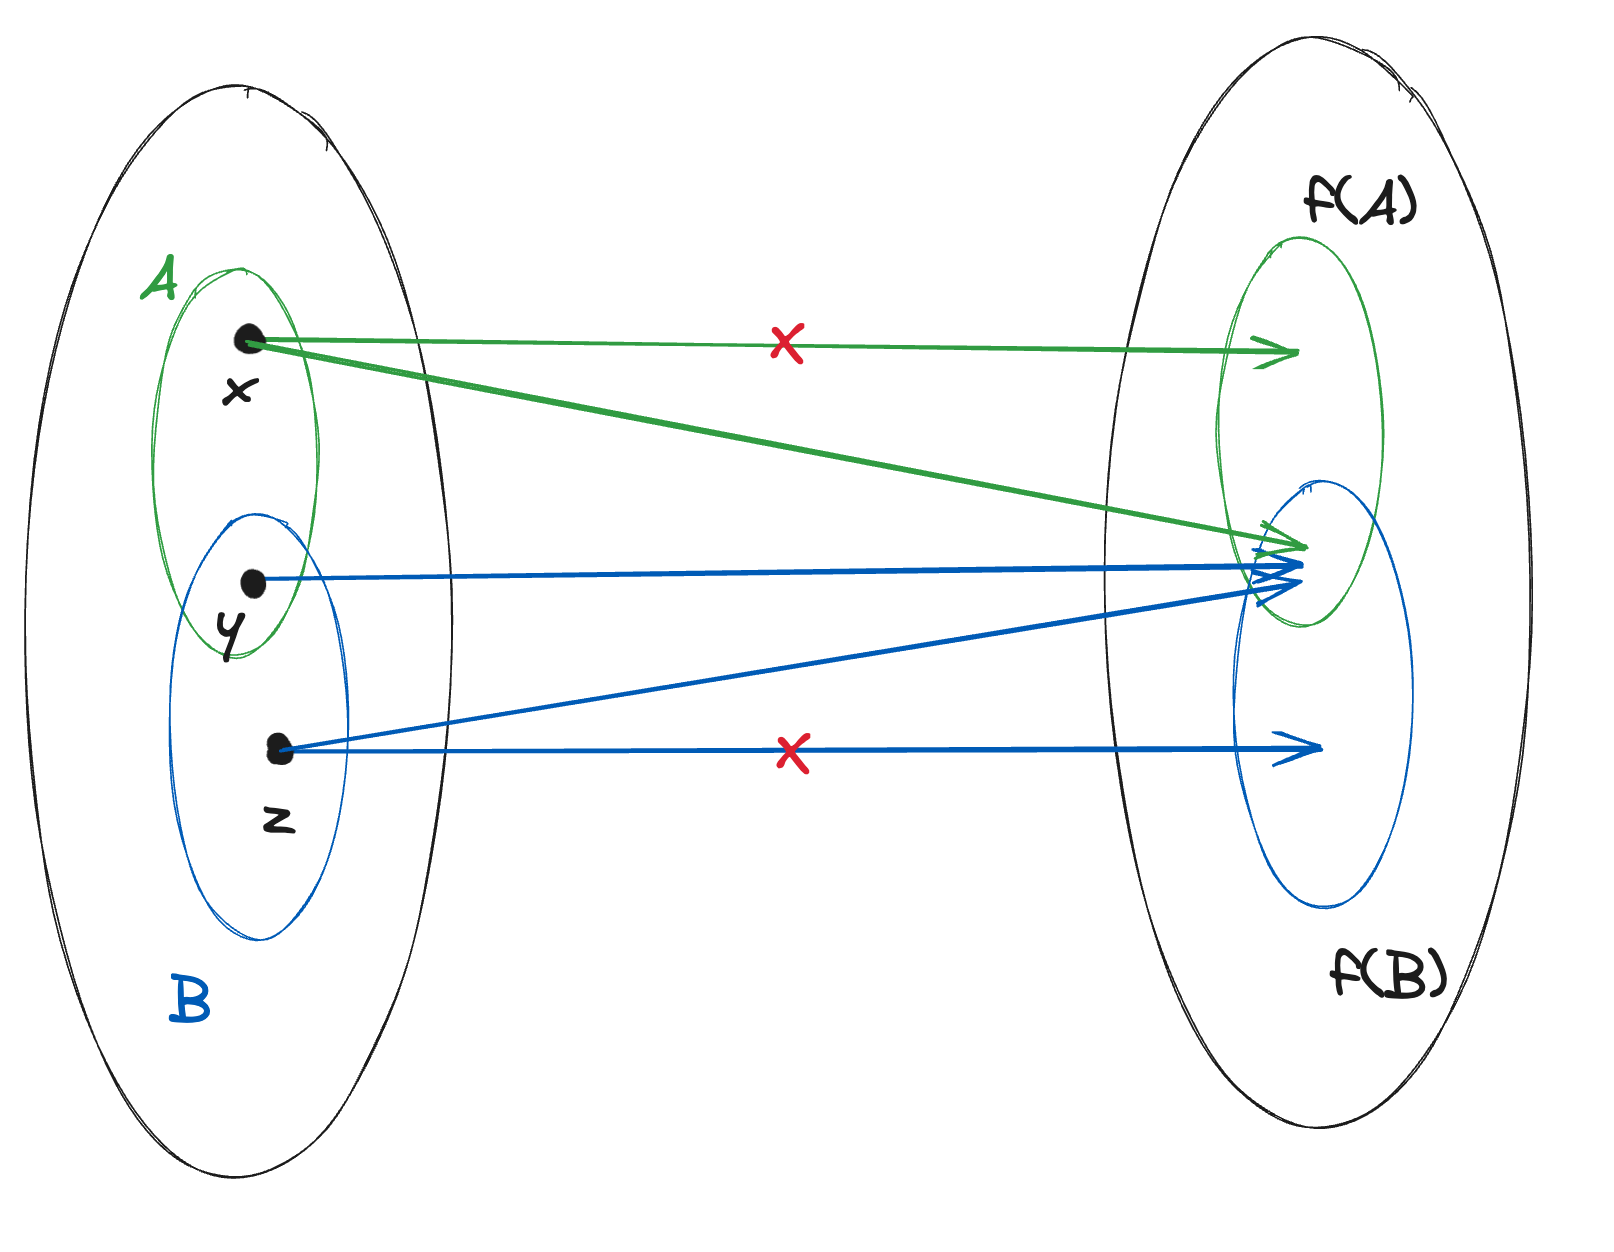
\includegraphics[width=125mm]{img1}\]

Докажем для $n \geq 1$, используя метод полной математической индукции. \sspace

\textbf{База:} \sspace 
$Z_1 = F_2 = 2$. Подойдут слова 0 и 1 - верно
\sspace
\textbf{Шаг:} \sspace
Рассмотрим слово длиной n, если оно оканичивается на 0, оно могло получиться из слов длиной n - 1, оканчивающихся на 1. Слов длиной n - 1, которые оканчиваются на 1 ровно столько же, сколько слов длиной n - 2 (потому что к любому слову можно доставить 1 в конце). \\
Если же слово длиной n оканчивается на 1, то оно могло получиться из любого слова длиной n - 1 (аналогично). Получается, что $Z_n = Z_{n - 1} + Z_{n - 2}$, используем предположение индукции, получим $Z_n = F_{n} + F_{n - 1} = F_{n + 1}$ \bs

\p
  Дайте комбинаторное доказательство равенства  
  $\ds
  \sum_{j=0}^k\binom{r}{j}\binom{s}{k-j} = \binom{r+s}{k}$.

Для простоты доказательства будем называть элементы из r буквами, а элементы из s цифрами. j проходит от 0 до k, то есть рассматриваются все возможные количества букв, остальные места занимают цифры. Дальше для каждого j выбираются все наборы из j букв и k - j цифр. То есть для каждого возможного количества букв перебираются все возможные наборы букв размера j и цифр размера k - j. Почему это равно $\mattwo{r + s}{k}$? Можно перефразировать последнюю запись как набор размера k, где каждый элемент это буква или цифра. Очевидно, что фиксируя количество букв не меняется итоговое количество наборов.
\end{document}
